\documentclass[a4paper,12pt]{extarticle}
\usepackage[top=3cm]{geometry}

\usepackage{titling}
\setlength{\droptitle}{12em}

\usepackage[scaled]{helvet}
\renewcommand\familydefault{\sfdefault} 
\usepackage[T1]{fontenc}
\usepackage{graphicx}
\usepackage{hyperref}

\usepackage[usenames, dvipsnames]{color}
\definecolor{mygray}{rgb}{0.5, 0.5, 0.5}
\definecolor{mygreen}{rgb}{0,0.6,0}
\definecolor{myblue}{RGB}{57, 135, 189}

\usepackage{listings}
\lstset{ 
    language=java,
    basicstyle=\ttfamily\footnotesize,
    keywordstyle=\color{myblue},
    commentstyle=\color{mygray},
    stringstyle=\color{mygreen},
    frame=single,
    showstringspaces=false,
}

\title{\textbf{Software Engineering\\\vspace{5mm} CPS2002\\\vspace{5mm}  Assignment Report}}

\author{\LARGE Martin Bartolo - 0218300L\vspace{1mm}\\ \LARGE Mikhail Cassar - 0319599M\vspace{3mm}\\ \large BSc (Hons) Computing Science and Mathematics}

\date{Assignment due 27\textsuperscript{th} May 2019}

\setcounter{secnumdepth}{0}

\begin{document}

\setlength{\parindent}{0pt}
\setlength{\footskip}{50pt}
\pagenumbering{arabic}

\maketitle
\thispagestyle{empty}
\newpage

\tableofcontents
\newpage

\section{Diagram Example}
\begin{center}
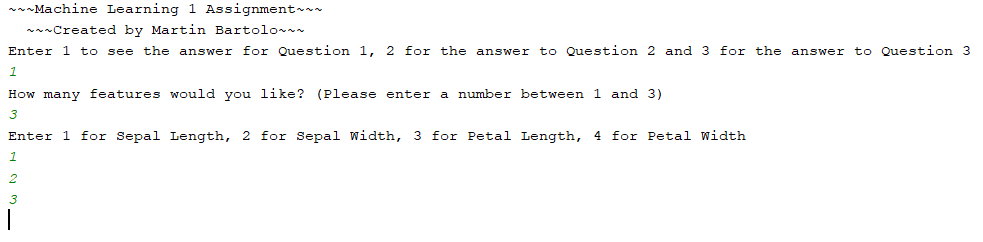
\includegraphics[width=\textwidth]{FigureExample.png}
\end{center}

\section{Code Snippet}
\begin{lstlisting}
public class Main{
  public static void main (String args[]){
    System.out.println("Hello World!");
  }
}
\end{lstlisting}

\section{Introduction}
The aim of this assignment was to collaboratively work on a software project, with the main focus being on rigorous software testing and the use of Git. Our first task was to set up our environments, namely our Git repository on Github and our Jenkins environment on the University Jenkins server. First, we initialised our Git repository and ensured that each team member could commit changes and push and pull them from Github. When this was ensured, we set up our Jenkins environment to work with Maven and scan for changes from Github every few minutes. Whenever changes are found, they are built and run with a detailed code coverage report and test results being displayed using the Emma plug-in. Our progress at this point can be seen by viewing the "Part1" tag on our Github repository. After completing our set-up, we were ready to face the 2 remaining tasks which will be discussed in detail throughout the remainder of this report.
\newpage


\end{document}